%\doublespacing 
\label{chapter2}
\section{Variety and Reptetition}
In response to Kyle Adams' seminal \textit{Music Theory Online} article ``Aspects of the Music/Text Relationship in Rap,'' Justin Williams litigated an important phenomenon in rap music production that changed alongside the move from the turntable to the recording studio. He writes:

\begin{quote}
    \small ``In terms of rap music recordings, the idea of a completely fixed loop is largely fictitious. There may be a set of layers which we could term the `basic beat' which repeats intact for certain durations of time, but one would be hard-pressed to find an entire musical complement that stays the same throughout. Rap music’s layers will more often than not fluctuate throughout a given song, with sonic additions and subtractions, manipulations of digital samples, and even sharp changes in aspects of the basic beat.''\footnote{\cite{justinawilliamsBeatsFlowsResponse2009}. It is worth noting that Adams does not necessarily dispute the occurrence of development within an accompaniment as a phenomenon, but he does maintain that the unchanging elements of the beat function as ``primary accompanimental layers'' (See \cite{kyleadamsPeopleInstinctiveAssumptions2009}.)}
\end{quote}

\noindent \normalsize As both a fan of and critical listener to rap music, I experience repetition and variation significantly within musical lexicon of the rap instrumental. Adams notes that even as the locus of rap music-making moved into the studio, producers remained adherent to the break-beat based origins of the genre, and so structural elements of the hip-hop beat tend to repeat within a four to eight bar, often simple quadruple metrical space. At the same time, Williams' observations point towards producers' observable preference for variation within repetition, made feasible by newer technologies for sampling, manipulating, and composing with pre-recorded digital materials.

The answer to whether the hip-hop beat is primarily repetitive or primarily developmental is indeterminate because both dimensions exert influence over the process of creating it. Instead, I want to interrogate how producers use these dimensions to aesthetic or rhetorical ends: to invoke Loren Kajikawa's notion of sounded phenomena in hip-hop, how ``rap artists produce (and listeners interpret) musical meanings at the level of the song.''\footnote{\cite{lorenkajikawaSoundingRaceRap2015}, 2.} While Kajikawa's focus on racial identity unpacks the most important element of a producer's  curatorial work, another conscious choice a producer makes is to identify with or against the hip-hop mainstream. Producers use the beat as a means of coding themes and identities complementary to the rapper who declares allegiance to the underground within their flow. Such a reading, I believe, resonates with the central argument of Kajikawa's \textit{Sounding Race} because ``rap has cultivated a mainstream audience\textellipsis by promoting highly visible (and often controversial) representations of black masculine identity''\footnote{\cite{lorenkajikawaSoundingRaceRap2015}, 5.}.

As with any sub-generic distinction predicated on narratives of authenticity, I use the term \emph{underground} trepidatiously, knowing full well it has as many meanings as it has users. What I call the underground signifies a space where deviation from the mainstream is expected. This is not a value judgement, nor an all-encompassing definition of either mainstream or underground. My definition is necessarily vague because these are elusive terms, but they hold importance because they represent \textit{de facto} ``imagined communities'' with which rappers, producers, and listeners identify.
\footnote{The concept of the imagined community of hip-hop has been broadly traced by Williams via Joseph G. Schloss: the term comes from Benedict Anderson's conceptualization of how a community Williams argues for the importance of recognizing hip-hop as an imagined community, a term coined by Benedict Anderson for conceptualizing nationalism, because such a community must exist to provide a cohesive set of strategies by which producers and listeners interpret musical objects (see \cite{justinawilliamsRhyminStealinMusical2013}: 13-19.) 

Joseph G. Schloss also develops the notion of an imagined hip-hop community to categorize the network of hip-hop producers who serve as his ethnographic subjects, and to explain their conception of the audience for their music (see \cite{josephgschlossMakingBeatsArt2004}: 4-5.)}

In this chapter, I argue that producers work with rappers to sound the hip-hop underground by using variety within their construction of the beat, punctuating alternative identity in sampling; I base this argument in transcriptions that illustrate developmental and repeating elements within the musical texture. My case studies show that underground producers tend to deviate from expectations concerning form in their sectional divisions of the beat. Highlighting sample-based and non-sample-based approaches to beat-making, I trace methods of sample and loop manipulation such as \emph{resampling (or recomposing)}, \emph{choking}, \emph{slipping}, \emph{glitching} as producers' means of variation. Lastly, I contend that underground hip-hop is sounded by an overarching aesthetic of disunity, linking the tradition to Olly Wilson's heterogeneous sound ideal of African-American music.

%\clearpage
\section{Methods of Transcription and Analysis}
I use transcription in this chapter\textemdash indeed, overall in this project\textemdash despite knowing that it introduces a level of abstraction from both the musical practice and perceptual experience of my hip-hop repertory. Scholars such as Joseph G. Schloss have meaningfully analyzed hip-hop production while eschewing transcription altogether on ethical and aesthetic grounds.\footnote{\cite{josephgschlossMakingBeatsArt2004}, 13-15.} Others, like Kajikawa and Adam Krims, have employed methods of transcription that move away from standard notation in Western Classical tradition.\footnote{\textit{Cf.} \cite{lorenkajikawaSoundingRaceRap2015}, 29-30 and 36-37; \cite{adamkrimsRapMusicPoetics2000}: 105-110.} Still others, including Adams and Robert Komaniecki, rely primarily on standard notation in order to present their arguments within traditional spheres of music-theoretical discourse.\footnote{\textit{Cf. }\cite{kyleadamsMetricalTechniquesFlow2009}; \cite{robertkomanieckiAnalyzingCollaborativeFlow2017}.} Each approach holds its own merit, and each privileges a different audience: the creator, the listener, and the academic.

Although I understand Schloss and others' reticence to transcribe rap music, my choice to do so grows out of the style of deep listening requisite to creating a transcription. By using transcription, I do not aim to apply ``the tools of notation and analysis developed for the study of Western Classical music\textellipsis uncritically to rap music.''\footnote{\cite{lorenkajikawaSoundingRaceRap2015}, 12.}. Instead, I offer them as a subjective realization of my ``living inside'' the musical object for a time.\footnote{\cite{peterwinklerWritingGhostNotes1997}: 200.} Transcription therefore offers the best method of communicating my experience with the music in a written medium.

I use both standard and non-standard styles of transcription in this chapter to represent the tendency to create variety within repetition in distinct ways. First, I use tables that I call ``roadmaps'' to overview musical form, noting the relationship between sections, samples, and durations.\footnote{Each roadmap in the chapter has a corresponding expanded version that details the function and relationship of each instrumental layer and counting durations by samples. These expanded versions can be found in the appendix beginning on p.~\pageref{appendix:fullroadmaps}.} I also pay special attention to when producers create variety within the musical texture using one of the four methods listed above, and defined below. In addition, I use standard notation to create a musical ``snapshot'' of the beat at distinct points in the musical texture. These ``snapshots'' allow me to discuss the function of particular musical layers and also to more closely analyze the methods of creating variety outlined in the roadmaps. Using staff notation requires a certain reduction of the rhythmic and textural complexity of my pieces, but I use these snapshots in an effort to draw out the moments that cannot be easily notated within them.

As my roadmaps show, underground producers play with expectations for form in mainstream hip-hop, typically avoiding the \emph{verse-hook} formal model. Ben Duinker defines verse-hook form in hip-hop as an analog to \emph{verse-chorus} paradigms in other areas of popular music, and he shows that hip-hop's assimilation to mainstream popular culture has correlated with the increase of this form.\footnote{\cite{benduinkerSongFormMainstreaming2020}, 105.} At the same time, he differentiates verse-hook from verse-chorus on account of the means by which hooks fulfill the role of refrains.\footnote{Duinker notes that, unlike choruses, hooks do not lend themselves to ordered pairings that David Temperley labels ``verse-chorus units'' or VCUs, nor do hooks use the same features of differentiation that Temperley notes in rock songs. See \cite{davidtemperleyMusicalLanguageRock2018}, 159\textit{ff}.} Nevertheless, the correlation between verse-hook form and the mainstreaming of rap music in popular culture offers underground producers a model of song form with which to converse in their effort to create hip-hop in dialogue with expectations.

The producers in my repertory tend to construct their beats in ways that sound the section types Duinker identifies\textemdash  hooks, instrumentals, and ``looser-organized'' vocal sections.\footnote{\cite{benduinkerSongFormMainstreaming2020}, 95-101.} At the same time, the function of a section based solely on production becomes problematic when an emcee through-composes their rapped text, as they often do in the repertory I examine. How a producer chooses to order musical material can either clarify or contrast the form projected by the vocal performance, and underground producers use form playfully in relation to what the emcee projects with their vocal performance.

My snapshots exhibit how underground producers treat variety within formal sections as aesthetically preferential to unaltered or layered loops and samples. Duinker notes that within verses particularly, the looped sequence of the beat can change gradually through the introduction or subtraction of loops that are generally one, two, or four measures in length.\footnote{\cite{benduinkerSongFormMainstreaming2020}, 96.} While producers often layer in new material in my repertory, they also use techniques that create drastic changes, even within a formal section. 

Specifically, underground producers introduce changes within the accompanimental beat layer using techniques that mimic the live, improvisatory roots of hip-hop; these are the methods of alteration I introduced above. In order to present my close readings of each case study below, I will define \emph{resampling (or recomposing)}, \emph{choking}, \emph{slipping}, \emph{glitching} up front.

I use the term resampling to encapsulate any changes a producer makes to a sample while still presenting it as a complete loop. The term reflects a function offered to producers who use samplers like the Roland SP series or Digital Audio Workstations like Ableton, where any audio can be played with post-processing effects and other manipulations while being captured on a new sample pad or audio track. This allows producers to make changes to the pitch of a sample, the rhythmic sequence of components within a sample, and the engagement of effects ``in real time'' based on previously recorded material, and thus becomes a method for altering pre-recorded material in hip-hop. Recomposing functions much like resampling but particularly for producers who record live or software instruments alongside samples. A recomposition occurs when a producer takes a repeated loop and alters its content, either with new pitch and rhythmic material or by changing some element of the loop's timbre. 

Sample choking deals with muting a portion of the loop or sample completely, cutting it off as a sound source. Compared to subtracting a sample from a mix, sample choking happens within the length of a single sample or loop. Sample chokes can occur at lengths perceptually experienced as a beat, as well as below the beat level beyond the point of being meaningfully notated. Like resampling or recomposing, choking plays with the perception of repetition within the loop but does not completely disrupt it.

In comparison, glitching and slipping challenge a listener's sense of the repetitive structure more drastically and clearly mark change to a repeating sonic objects in mix. Glitching takes a portion of a sample or loop and ``chops'' it, then repeats the selected portion, often stretching portions of audio shorter than a beat to take up space larger than a beat. Glitching interrupts the musical texture in a way comparable to scratching a vinyl record would in turntabling. Slipping, by contrast, disturbs repetition much more subtly: slipping occurs when two samples of slightly varied lengths loop over long lengths of time, widening the space between them. Alternatively, producers slip samples through expressive, delayed re-triggering of samples. Both methods create a disalignment of sample and loop onsets.

As my analyses below demonstrate, underground producers use these compositional techniques to create variety within the sonic profile of their beats. In both sample-based and non-sample based approaches to beatmaking, underground producers create beats that are internally and formally varied, and do so in dialogue with the emcee's vocal delivery. Their use of these techniques, along with the formal trajectory of their beatmaking, introduce heterogeneity to the musical work, and therefore ultimate sound as underground in comparison to more mainstream approaches to form and beatmaking.
%\clearpage
\section{Sample-Based Case Studies}
 As Tricia Rose notes, the contemporary practice of sample-based beatmaking links back to hip-hop's origins, echoing the practice of looping breakbeats on the instrumental b-sides of vinyl records pioneered by DJs like Kool Herc and Grandmaster Flash.\footnote{\cite{triciaroseBlackNoiseRap1994}, 51.} Because producers who sampled do not need to be a multi-instrumentalists to create a full musical texture, sample-based beatmaking democritizes the music production; but furthermore, it imbues hip-hop with a sonic lineage and particular type of nostalgia. Rose likens the ingenuity of hip-hop production to other forms of Black creativity, where making something good often involved ``making\textellipsis out of the scraps\textemdash creating a delicacy of the undesirable, discarded parts.''\footnote{\cite{triciaroseHipHopWarsWhat2008}, 264.} In the underground, the process of selecting a sample, re-contextualizing it in a new space, and exploring the full extent of variety it may hold seems to be a look backwards to this tradition, and thus a way of honoring a broader history of the ingenuity of Black Americans.

\phantomsection
\subsection*{\centering MF DOOM's ``One Beer''} 
\addcontentsline{toc}{subsection}{MF DOOM's ``One Beer''}

    \begin{table}[ht]
        \centering
            \begin{tabular}{|c|c|c|c|l|}
                 \hline
                  Section         & Timecode & Duration & Sample              & Note                    \\ \hline
                  Intro           & 0:00     & 8 Bars   & ``Huit Octobre'' I  & Choked in Bar 8         \\ \hline
                  Verse 1A        & 0:20     & 16 Bars  & ``Huit Octobre'' II &                         \\ \hline
                  Verse 1B        & 1:02     & 16 Bars  & ``Huit Octobre'' II & Choked in Bar 0.4       \\ \hline
                  \sout{Hook}     & 1:43     & 8 Bars   & ``Huit Octobre'' I  & Choked in Bar 8.3-4     \\ \hline
                  Verse 2B        & 2:03     & 8 Bars   & ``Huit Octobre'' II & Choked in Bar 0.4, 8.4  \\ \hline
                  \sout{Verse 2C} & 2:24     & 16 Bars  & ``Huit Octobre'' II & Choked in Bar 0.4       \\ \hline
                  Skit            & 3:06     & 26 Bars  & \textit{Spider-Man} & Resampling, drum improv \\ \hline
             \end{tabular}
        \caption{Condensed Roadmap to MF DOOM and Madlib's ``One Beer.''}
        \label{tab:onebeer}
    \end{table}

Madlib produces ``One Beer'' using two samples from the French funk band Cortex's ``Huit Octobre 1971.'' Outlined in Table~\ref{tab:onebeer}, Madlib sequences these two samples with a somewhat normative approach to form, in contrast to DOOM's through-composed verse. Madlib starts ``One Beer'' with 8-bar introduction built from the first sample, followed by two 16-bar verse parts built from the second. He then switches back to the first sample, making space for a hook, but DOOM's verse continues over this projected boundary. After 8 bars, the second sample re-enters for another 24 bars, creating a nearly parallel second verse area for DOOM's verse. Madlib and DOOM project contrasting forms in their respective roles as producer and rapper, and the dissonance between the two creates introduces heterogeneity between the text and the instrumental.

    \begin{figure}[ht]
        \centering
        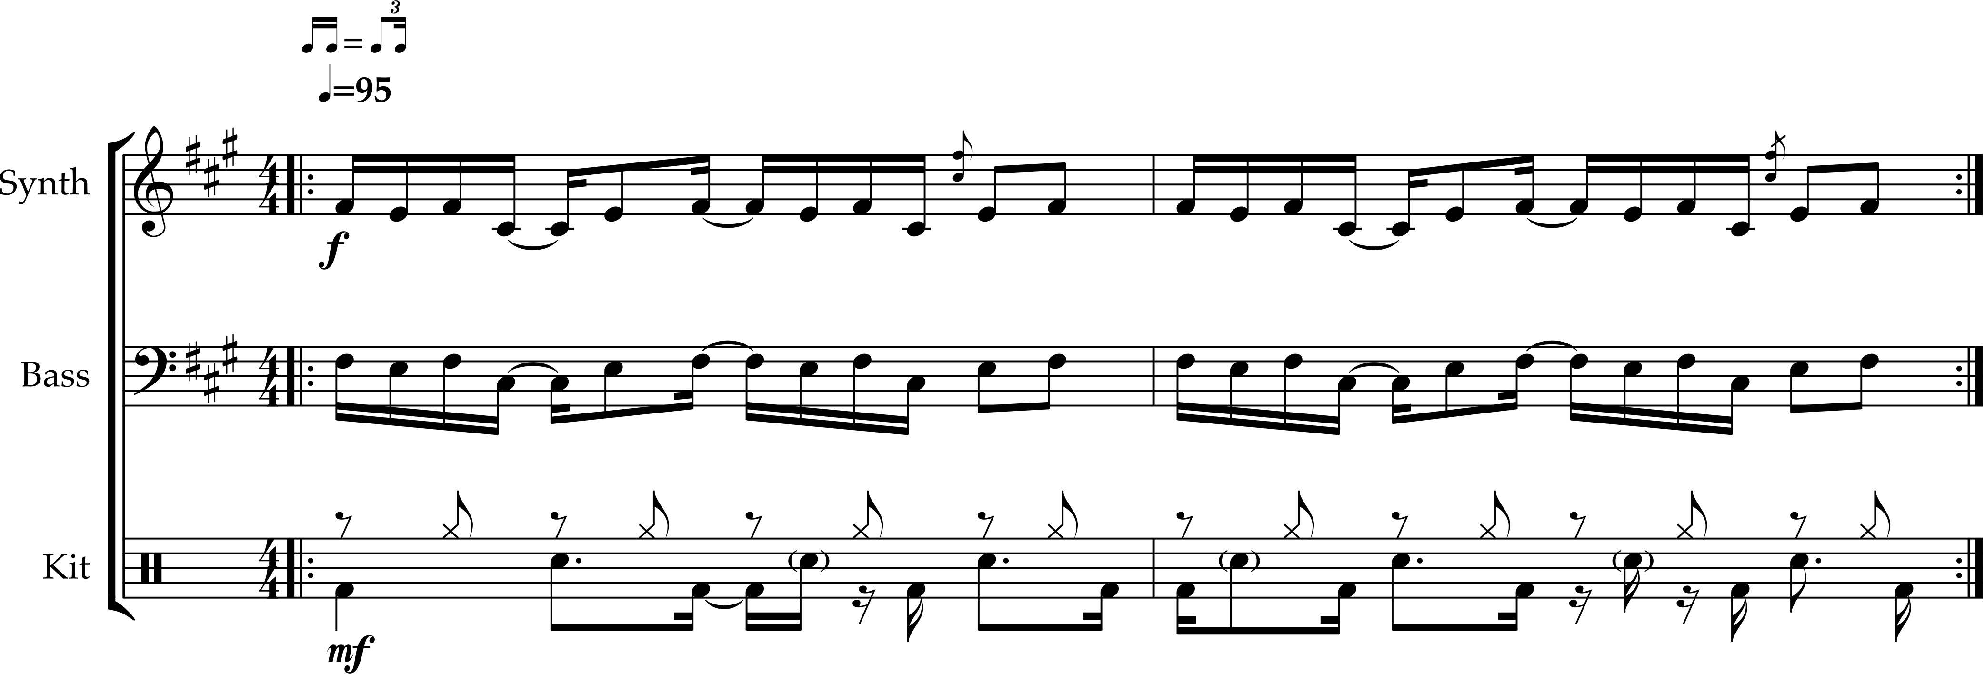
\includegraphics[width=\textwidth]{images/figures/chp 02/000019onebeerintro.pdf}
        \caption{Snapshot of Madlib's first sample in ``One Beer,'' 0:00-0:19.}
        \label{fig:onebeerintro}
    \end{figure}

Madlib also introduces heterogeneity within the beat itself, primarily through musical disparity in the selection of sampled portions from ``Huit Octobre.'' His first selection, 1:58-2:09 of Cortex's recording, is pitched up a whole step and slightly sharper than a quarter tone,
tonicizing F-sharp. Shown in Figure-\ref{fig:onebeerintro}, the sample grooves in a triplet eighth swing, featuring synth and bass in octaves arpeggiating I$^{b7}$ and a skeletal drum part emphasizing backbeats. When the track returns to the first sample, the relative stasis of the musical elements grant the sample a hook-like function.

The first sample sounds hook-like in nature for two reasons. First, it is texturally distinct from the sample which underscores the verse portion of ``Huit Octobre,'' the primary instrumental criterion Duinker identifies for distinguishing hooks from verses.\footnote{\cite{benduinkerSongFormMainstreaming2020}, 99.} Second, it is created from a shorter, more singularly-focused musical idea. Its harmony, which Adams typifies as \emph{repetitive}, is created from two parts arpeggiating a one-measure idea in rhythmic unison, only with slightly varied articulations in each statement.\footnote{\cite{kyleadamsHarmonicSyntacticMotivic2020}. The three categories Adams provides for harmony in hip-hop are repetitive, oscillating, and expansional, all of which I touch on throughout the course of this chapter.} Overall, the first sampled section is less busy in texture and musical material, making it sound like a point of arrival when Madlib brings it back.

Madlib contrasts the first sample with his selection of the second, 0:23-0:25 of the Cortex recording. Although also pitched up slightly sharper than a whole step, this portion is slower and has a straight rhythmic feel. As Figure~\ref{fig:onebeermain} shows, both the overall musical texture and harmonic content of this sampled section have thickened in comparison to the first. Playing distinct and more typical instrumental roles, the bass and synth underscore a vocal part singing nondescript syllables and create oscilatting extended tertian chords on G major and F-sharp minor.

    \begin{figure}[ht]
        \centering
        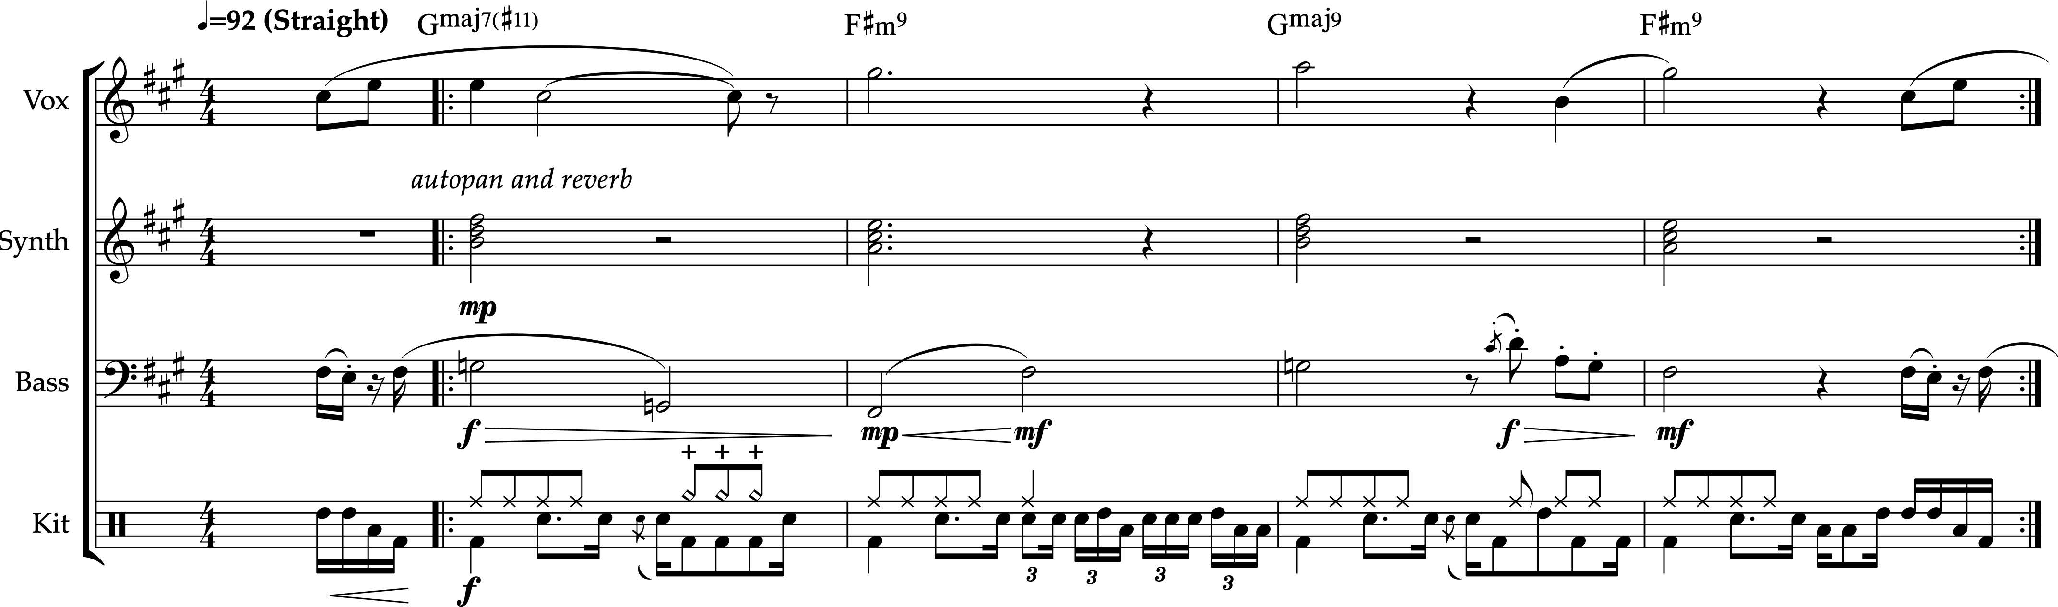
\includegraphics[width=\textwidth]{images/figures/chp 02/020031onebeermain.pdf}
        \caption{Snapshot of Madlib's second sample in ``One Beer,'' 0:20-0:31.}
        \label{fig:onebeermain}
    \end{figure}

Perhaps the most prominent shift in texture comes with the rhythmic complexity of the drum part in the second sample. Like the fuller harmony, the drums fill up sonic space using distinctive fills and striking timbres throughout the four bar loop; this culminates in the prominence of the two-beat long triplet eighth fill in m. 2 of Figure~\ref{fig:onebeermain}. As Schloss notes, producers often choose their samples based on the aesthetic delight they experience concerning timbre, and that drum sounds are sought after with preference.\footnote{\cite{josephgschlossMakingBeatsArt2004}, 141-142.} Certainly, this second section luxuriates in the sonic quality of the drum part.

Comparing the texture, harmony, and groove of each of Madlib's samples illustrates how internally varied ``One Beer'' is, even simply through the process of sample selection. Although makes use of some of the methods of altering the sample\textemdash particularly, choking the sample to delineate sectional transitions\textemdash his primary method of introducing variety in the main part of ``One Beer'' is through the juxtaposition of the two lead samples. Juxtaposing musical elements in this manner aligns with Wilson's heterogeneous sound-ideal, particularly because of the resulting rhythmic clash and  timbral stratification across sample boundaries.\footnote{\cite{ollywilsonHeterogeneousSoundIdeal1992}, 328-329.}
\phantomsection
\subsection*{\centering Kendrick Lamar's ``Rigamortis''}
\addcontentsline{toc}{subsection}{Kendrick Lamar's Rigamortis}
    \begin{table}[ht]
        \centering
            \begin{tabular}{|c|c|c|c|l|}
                \hline
                Section  & Timecode & Duration & Sample        & Note \\ \hline
                Intro    & 0:00     & 4 bars   & ``The Thorn'' & \\ \hline
                Hook     & 0:10     & 6 bars   & ``The Thorn'' & Full sample plays \\ \hline
                Verse 1A & 0:27     & 12 bars  & ``The Thorn'' & \\ \hline
                Verse 1B & 0:59     & 10 bars  & ``The Thorn'' & Improvisatory sample choking \\ \hline
                Hook     & 1:26     & 6 bars   & ``The Thorn'' & Lead sample slips backwards \\ \hline
                Verse 2A & 1:43     & 6 bars   & ``The Thorn'' & \\ \hline
                Verse 2B & 2:04     & 8 bars   & ``The Thorn'' & Alternating sample choking \\ \hline
                Hook     & 2:31     & 6 bars   & ``The Thorn'' & Improvisatory sample choking\\ \hline
            \end{tabular}
        \caption{Condensed roadmap to Kendrick Lamar and Willie B's ``Rigamortis.''}
        \label{tab:rigamortis}
    \end{table}

The production team for ``Rigamortis''\textemdash Willie B and Sounwave\textemdash use Willie Jones III's ``The Thorn'' as the lead sample for the track. The team samples 0:13-0:20 of an up-tempo jazz track, where the combo groups simple quadruple meter into 3+3+2 beat divisions to underscore a saxophone and trombone theme; this texture is detailed in Figure~\ref{fig:thethornfull}.

    \begin{figure}[ht]
        \centering
        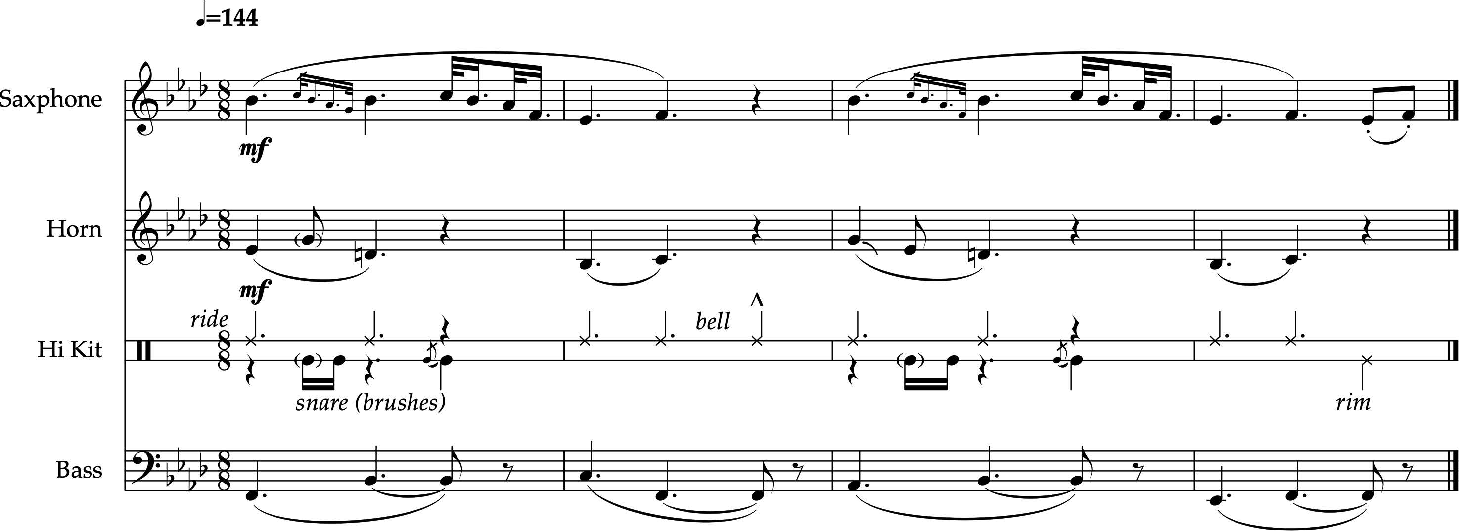
\includegraphics[width=\textwidth]{images/figures/chp 02/013020thethornfull.pdf}
        \caption{Snapshot of the sampled portion of ``The Thorn,'' 0:13-0:20.}
        \label{fig:thethornfull}
    \end{figure}

``Rigamortis'' begins with a nearly unadulterated triggering of the first two measures of the sample. The only changes the producers make are filtering out the low end and pitching the sample up slightly sharper than four semitones. In its new context, the two-bar phrase sounds as a one-bar unit within a down tempo hip-hop context. This is confirmed when, as shown in Table~\ref{tab:rigamortis}, the full four-measure sample is presented beneath Lamar's hook as a two-bar unit. Within the first verse, Willie B and Sounwave also layer in a drum sequence and sub bass drone on a low A using a filter sweep to demarcate their entrances. Figure~\ref{fig:rigamortisnoslip} snapshots the primary instrumental elements in the first verse section, which repeat largely unchanged from 0:43-0:55, with only slight choking of the lead sample.

\begin{figure}[ht]
    \centering
    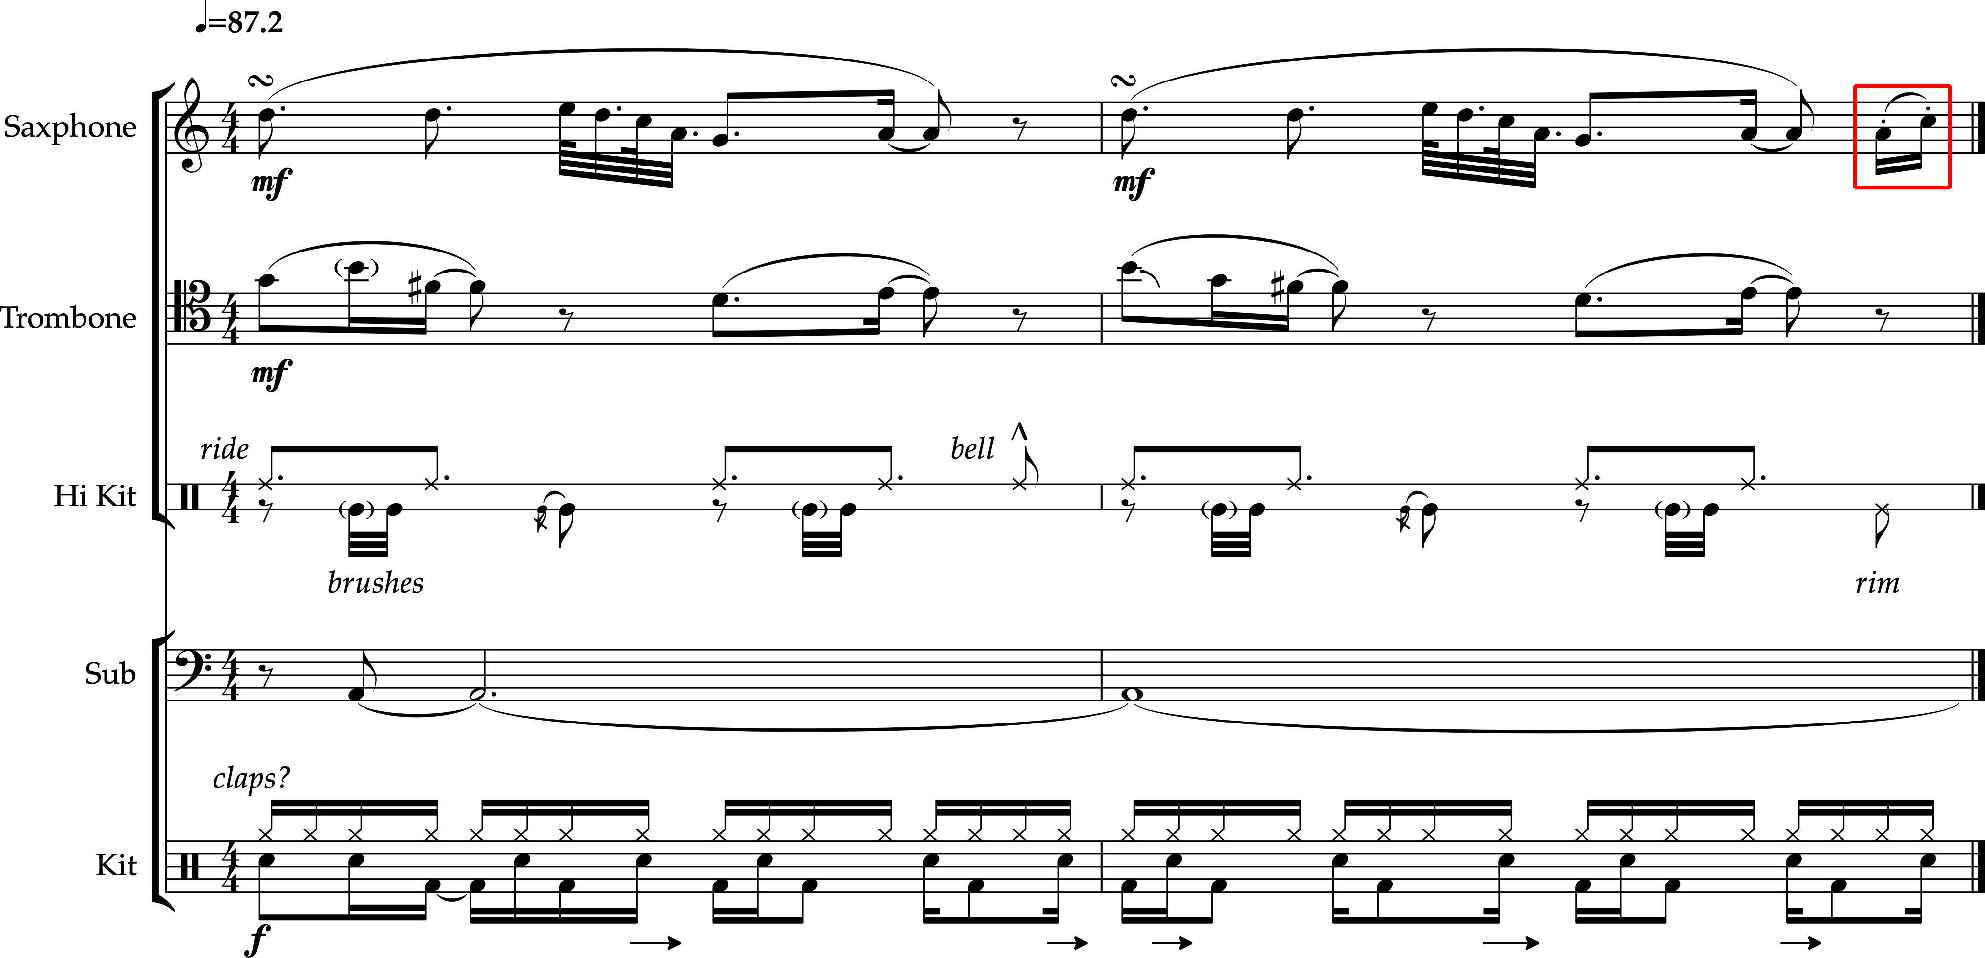
\includegraphics[width=\textwidth]{images/figures/chp 02/043053rigamortusnoslip.pdf}
    \caption{Snapshot of the first verse in ``Rigamortus,'' 0:43-0:55.}
    \label{fig:rigamortisnoslip}
\end{figure}

With these new musical elements, the producers recontextualize the harmony in ``The Thorn'' to what Adams refers to as \emph{repetitive}\footnote{\cite{kyleadamsMetricalTechniquesFlow2009}.} harmony that primarily sounds an a minor tonic function within a simple quadruple groove. The sample, drum, and bass each help ground the listener within Lamar's complex vocal delivery. In particular, Lamar plays with listener expectations about the function of repeated text: the call-and-response ``He dead!'' vocal track interrupts the continuity of Verse 1, splitting it into two verse parts. He also repeats the ``Got me breathin''' hook text as the beginning of the second verse after its return in the second hook. Lamar's vocal style also embodies heterogeneity because of its ``tendency to fill up the musical space'' within the mix, particularly when he transitions into to a more rapid rhythmic mode and higher pitch level within Verse 2B.\footnote{\cite{ollywilsonHeterogeneousSoundIdeal1992}, 328.} Willie B and Sounwave thus complement Lamar's vocal complexity with discrete, simplistic musical elements.


Although the presentation of these elements is straightfoward, Willie B and Sounwave constantly vary the samples and loops to inroduce variety subtly within the repetitive texture. The primary method they employ is \emph{slippage} of the lead sample backwards in the grid. Figure~\ref{fig:rigamortusslip} shows the disalignment of the lead sample with the overall groove. Both the drum sequence and Lamar's call-and-response vocal articulate a downbeat which the lead sample enters behind by two sixteenths; the producers also accent this position in the grid with a re-articulation of the sub-bass (with the sample). The lead sample now shifted back, the pickup figure which ends the lead sample now aligns with the next downbeat in the drums, thus complicating the perception of these loops as simple repetitions.

\begin{figure}[ht]
    \centering
    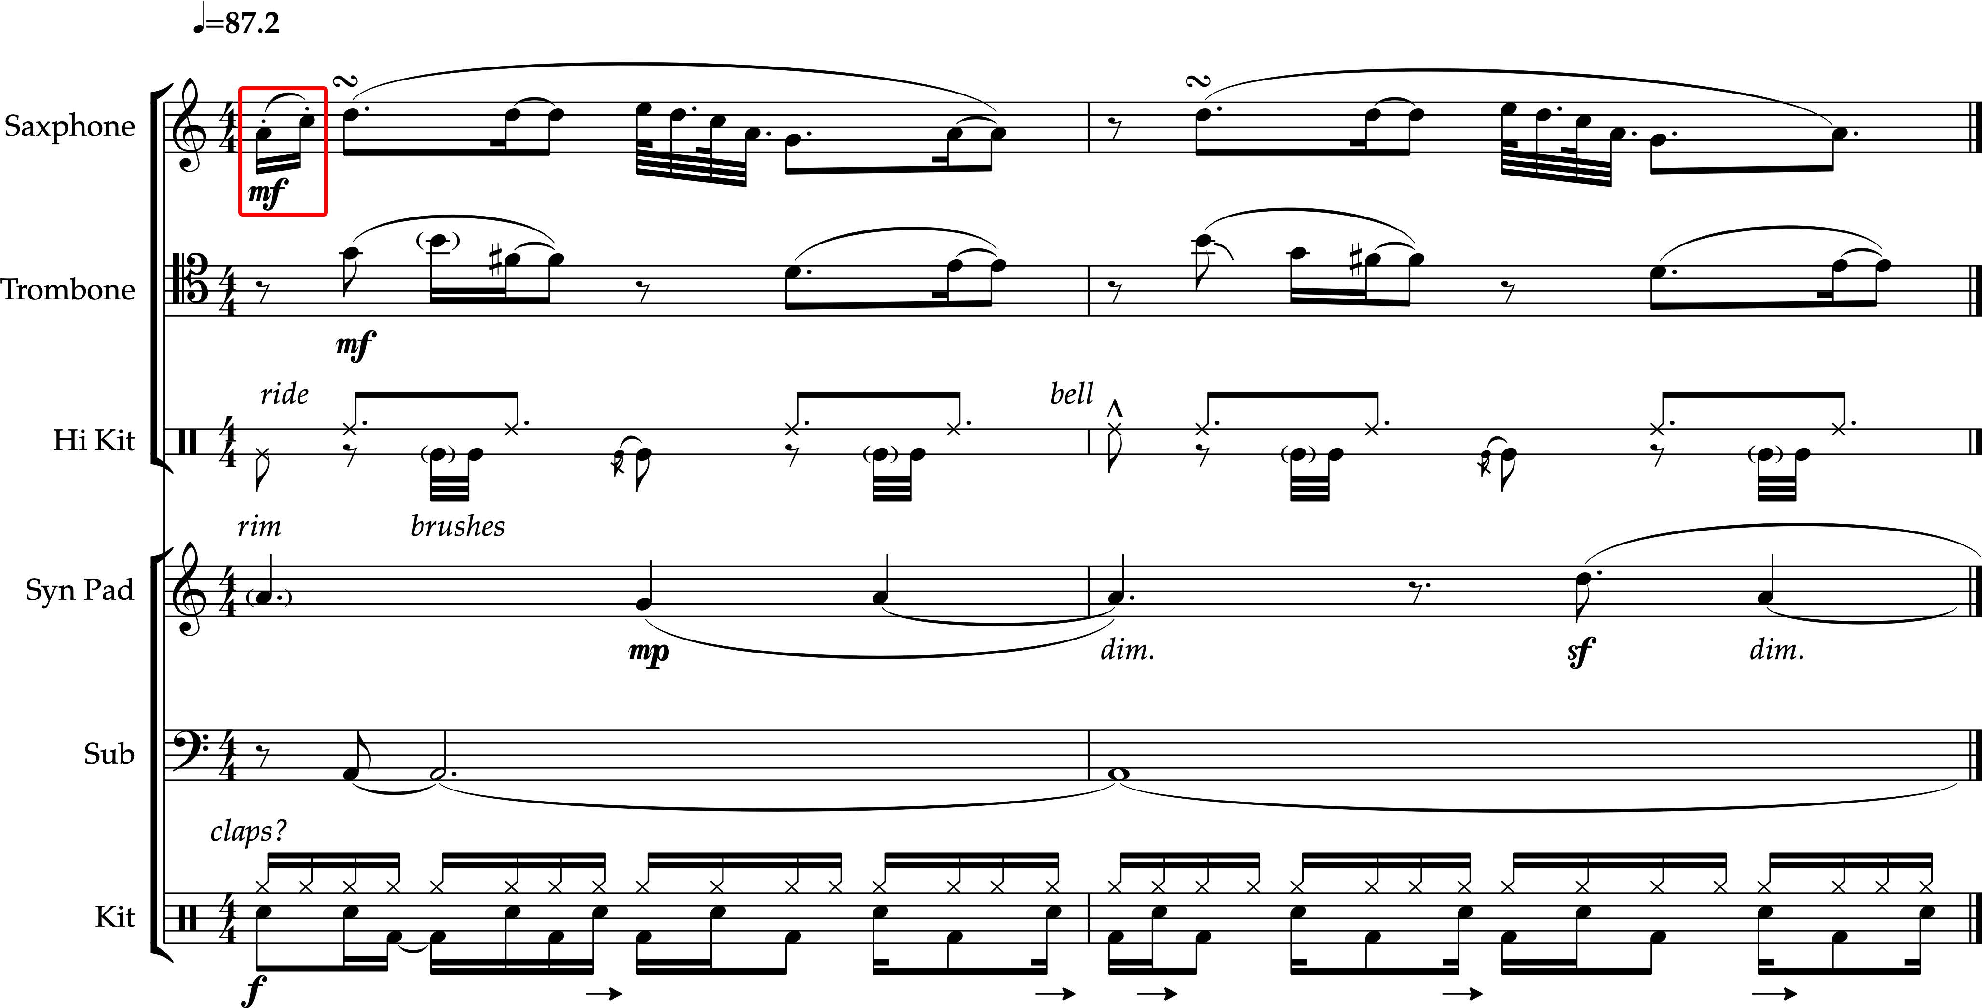
\includegraphics[width=\textwidth]{images/figures/chp 02/126137rigamortusslip.pdf}
    \caption{Snapshot of the first hook in ``Rigamortus,'' 1:26-1:37.}
    \label{fig:rigamortusslip}
\end{figure}

%The grounded, repetitive simplicity of the beat does not mean the beat is unchanging. Willie B makes frequent use of sample choking, evening muting the sample completely for parts of Lamar's final verse. He also obfuscates the texture by employing what I call \emph{sample slippage}, wherein the micro-rhythmic space between the lead sample and drum loop ebbs and flows due to slightly varied loop lengths and expressively delayed re-triggering.\footnote{The phenomenon of sample slippage dovetails with Anne Danielsen's work on the Beat Bin and rhythmic tolerance (see \cite{annedanielsenHereThereEverywhere2016}: 29\textit{ff.})} The affect of such shifting creates a listening experience akin to phasing, as samples (albeit sonically discrete ones) move in and out of sync with each other.  While Figure~\ref{} and Table~\ref{tab:rigamortis} show all of the sample loops beginning and ending in alignment, in reality, the beginnings and ends of loops are messy, and each float in and out of time with each other throughout the track.

%This devotion to messiness manifests heterogeneity within the limitations of a four-measure loop. The concepts of downbeat, meter, and formal structure are all fraught within ``Rigamortis,'' in a manner that echoes the technological limitations of rap's advent as a genre. Because of this messiness, ``Rigamortis'' sounds how one might expect a mixtape from Compton to sound, reinforcing Lamar's identity with the underground and his roots.

%\phantomsection 
%\subsection*{\centering Milo and Self Jupiter's ``Ornette's Swan Song''}
%\addcontentsline{toc}{subsection}{Milo and Self Jupiter's ``Ornette's Swan Song}

%\clearpage
\section{Live-Tracked Case Studies}
%The final two case studies investage Milo's 2015 `Rabblerouse,'' produced by Kenny Segal, and Noname's 2018 ``Blaxploitation,'' produced by Phoelix. Neither Segal nor Phoelix use a single lead sample to construct their beat; instead, they live-track their loops with instruments at their disposal. Both producers remain conceptually adherent to the basic beat, and both introduce variety using similar techniques for manipulation to sample-based approaches. Each producer varies the form of their beat against a conceptually mainstream structure, using vocal samples and musical styles to communicate alterity.

\phantomsection
\subsection*{\centering Milo's ``Rabblerouse''}
\addcontentsline{toc}{subsection}{Milo's ``Rabblerouse''}

\begin{table}[ht]
    \centering
        \begin{tabular}{|c|c|c|c|l|}
             \hline
            Section & Timecode & Duration & Sample                  & Note \\ \hline
            Intro   & 0:00     & 4 Bars   &                         & Rhodes extends over boundary \\ \hline
            Verse   & 0:08     & 24 Bars  &                         & Rhodes slips backwards \\ \hline
                    & 0:14     &          &                         & Drum glitch shifts downbeat \\ \hline
                    & 0:39     &          &                         & Drum glitch and bass recomp. \\ \hline
            Outro   & 0:56     & 4 Bars   &                         & Glich, recomp., and choking \\ \hline
                    & 1:03     &          & \textit{Soul Caliber} 2 & \\ \hline
        \end{tabular}
    \caption{Condensed roadmap to Milo and Kenny Segal's ``Rabblerouse''}
    \label{tab:rabblerouse}
\end{table}

On ``Rabblerouse,'' Milo delivers a single 24-bar verse that operates as an introductory song fragment to the concept album it resides upon. Segal constructs an unstable beat, propelling the listener toward a resolution that arrives with the second track, ``Souvenir.'' The beat ends with a lone vocal sample of the character Yoshimitsu from \textit{Soul Caliber 2} to connect the two tracks. The sample also connects thematically to the penultimate track ``Napping Under the Echo Tree,'' when Milo refers to himself as the ``Yoshimitsu of Boyle Heights.''

    \begin{figure}[ht]
        \centering
        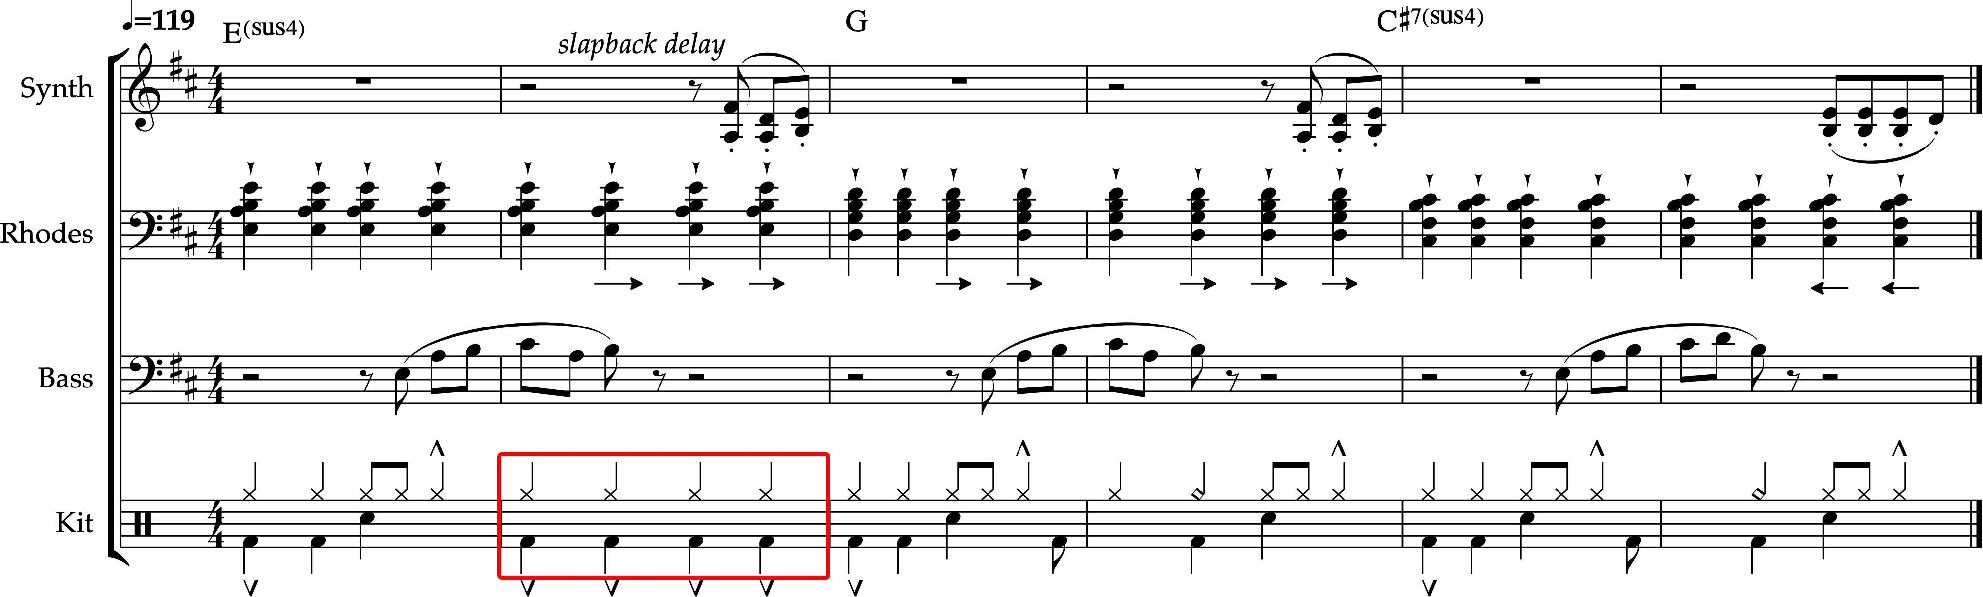
\includegraphics[width=\textwidth]{images/figures/chp 02/012023rabblefirstglitch.pdf}
        \caption{Snapshot of the first drum glitch in ``Rabblerouse,'' 0:12-0:23.}
        \label{fig:rabblefirstglitch}
    \end{figure}

Segal manifests instability in the beat for ``Rabblerouse'' on several structural levels. First, the loop repeats an irregular six-bar chord progression on a Fender Rhodes. The pattern, though technically \emph{expansional}, sounds unresolved.\footnote{\cite{kyleadamsHarmonicSyntacticMotivic2020}. Adams does not make it a requisite condition of the expansional harmonic category to function as a complete phrase, although he notes that it commonly will.} Figure~\ref{fig:rabblefirstglitch} indicates my harmonic reading: the chords function in E Dorian, but the progression leaves out a resolution to F-sharp minor that would close the loop.

``Rabblerouse'' also feels unstable because Milo's verse enters after four bars, and though this is conventional, the six-bar structure of the basic beat offsets the meters being projected by rapper and producer. Segal acccounts for this metric dissonance by repeating the loop six times, shortening the penultimate repetition to four bars to realign the verse's end with the next downbeat. Thereafter, he employs a \emph{sample glitch} where the downbeat is re-triggered four times in a row, extending the E$^{sus4}$ harmony. As Table~\ref{tab:rabblerouse} illustrates, the unresolved sonority heard from the beginning dissipates as the Yoshimitsu sample is triggered.


\normalsize Segal's fragmentary aesthetic on ``Rabblerouse'' sounds as a mode of alterity because it is uncommon for a hip-hop beat not to function as a closed loop. The metric dissonance projected from the beginning does not resolve by the track's end, necessarily drawing a listener in to the text function and pointing towards the remaining tracks on the album. This beat is unstable alone, but functions cohesively with the sonic palette of Milo's LP \textit{So The Flies Don't Come} as a whole. This technique is predicated upon an interest in lyricism and conceptual unity propagated within the underground hip-hop scene.

\phantomsection
\subsection*{\centering billy woods' ``Checkpoints''}
\addcontentsline{toc}{subsection}{billy woods' ``Checkpoints''}

\begin{table}[ht]
    \centering
    \begin{tabular}{|c|c|c|l|}
        \hline
         Section      & Timecode & Duration & Note                          \\ \hline
         Intro        & 0:00     & 8 Bars   & Guitar anacrusis choked       \\ \hline
         Verse I      & 0:26     & 22 Bars  & Vocal anacrusis               \\ \hline
                      & 0:40     &          & Guitar, synth recomp          \\ \hline
                      & 1:06     &          & Synth, drum recomp            \\ \hline
         Interlude I  & 1:40     & 4 Bars   &                               \\ \hline
         Hook?        & 1:51     & 4 Bars   & All parts anacrusis           \\ \hline
         Interlude II & 2:06     & 4 Bars   &                               \\ \hline
         Verse II     & 2:20     & 15 Bars  & Synth anacrusis glitch        \\ \hline
         
    \end{tabular}
    \caption{Condensed roadmap to billy woods and Kenny Segal's ``Checkpoints.''}
    \label{tab:checkpoints}
\end{table}


\section{The Co-Creation of Alternative Identity}
This paper has highlighted some of the ways in which heterogeneity, cohesion, development, and repetition can be mapped into the architecture of underground hip-hop beats. Producers code these phenomena into their music in myriad ways: elements of production that unify the sounded underground are alterations of verse and hook lengths and forms, manipulations of recorded material at the sample level, and additions of musical and textual signifiers alongside the emcee's flow. Via transcriptions that demonstrate both a beat's capacity for development and its repetitive structural layers, I concluded that producers and their beats play a coequal part to the rapper in demonstrating the alterity of underground identity. Future iterations of this project, however, will necessarily turn toward the role of the rapper in sounding the underground.